\section{Durchführung}
\label{sec:Durchführung}
\subsection{Versuchsaufbau}
Zentral in diesem Versuch ist die Röntegnestrahlung welche durch eine Öffnung an der Mantelfläche eines Zylinders, in dessen Mitte das Probenstäbchen sitzt, auf die Probe gestrahlt wird und dahinter gestreut wird. Die Innenseite des Mantels des Metallzylinders ist vollständig mit einem Film bedeckt.
Die Achse des Probenstäbchens steht senkrecht auf den beiden Deckeln des Zylinders. Eine schematische Skizze das Aufbaus ist in \ref{fig:Aufbau} gegeben.
\begin{figure}
	\centering
	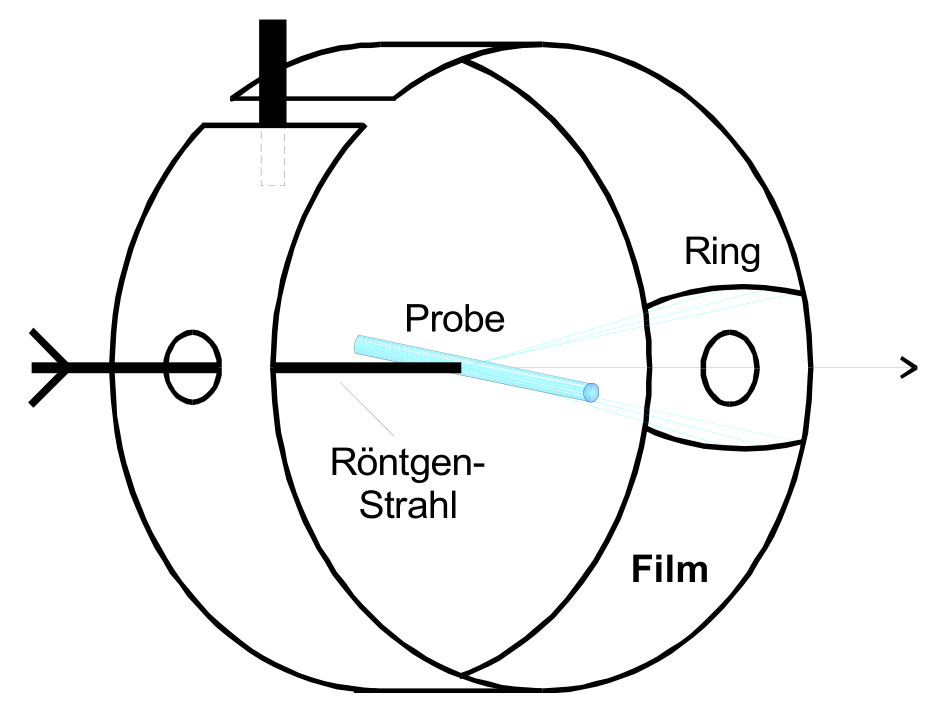
\includegraphics[width = \textwidth]{Abbildungen/Aufbau.png}
	\caption{kjhbfwrf \cite{Anleitung}. }
	\label{fig:Aufbau}
\end{figure}  
Der ganze Zylinder ist bis auf die Öffnung für die Röntgenstrahlung Lichtdicht verschlossen.
außen am Zylinder, an der Fassung des Probenstäbchens ist ein Motor angebracht, mit dem die Probe gedreht wird. 
Die Fassung selber ist so justierbar, dass das Probenstäbchens möglichst mittig zur Öffnung des Röngenstrahls steht.\\
Die Röntgenstrahlen werden durch eine Röntgenröhre erzeigt, welche eine Kupferanode besitzt.
Die BEschelunigungsspannung ist dabei deutlich gräßer, als die Kathodenspannung und beträgt \SI{40}{\kV}. 
Dabei werden die charakterisctischen Emissionslinien K$_{\alpha 1}$, K$_{\alpha 2}$ und K$_\beta$ erzeugt. 
Die K$_\beta$-Linie ist ncht relevant.  


\subsection{Entwicklung der Filme}








